\documentclass[dvipdfmx,a4paper,11pt]{article}
\usepackage[utf8]{inputenc}
%\usepackage[dvipdfmx]{hyperref} %リンクを有効にする
\usepackage{url} %同上
\usepackage{amsmath,amssymb} %もちろん
\usepackage{amsfonts,amsthm,mathtools} %もちろん
\usepackage{braket,physics} %あると便利なやつ
\usepackage{bm} %ラプラシアンで使った
\usepackage[top=30truemm,bottom=30truemm,left=25truemm,right=25truemm]{geometry} %余白設定
\usepackage{latexsym} %ごくたまに必要になる
\renewcommand{\kanjifamilydefault}{\gtdefault}
\usepackage{otf} %宗教上の理由でmin10が嫌いなので


\usepackage[all]{xy}
\usepackage{amsthm,amsmath,amssymb,comment}
\usepackage{amsmath}    % \UTF{00E6}\UTF{0095}°\UTF{00E5}\UTF{00AD}\UTF{00A6}\UTF{00E7}\UTF{0094}¨
\usepackage{amssymb}  
\usepackage{color}
\usepackage{amscd}
\usepackage{amsthm}  
\usepackage{wrapfig}
\usepackage{comment}	
\usepackage{graphicx}
\usepackage{setspace}
\usepackage{pxrubrica}
\usepackage{enumitem}
\usepackage{mathrsfs} 

\setstretch{1.2}


\newcommand{\R}{\mathbb{R}}
\newcommand{\Z}{\mathbb{Z}}
\newcommand{\Q}{\mathbb{Q}} 
\newcommand{\N}{\mathbb{N}}
\newcommand{\C}{\mathbb{C}} 
\newcommand{\Sin}{\text{Sin}^{-1}} 
\newcommand{\Cos}{\text{Cos}^{-1}} 
\newcommand{\Tan}{\text{Tan}^{-1}} 
\newcommand{\invsin}{\text{Sin}^{-1}} 
\newcommand{\invcos}{\text{Cos}^{-1}} 
\newcommand{\invtan}{\text{Tan}^{-1}} 
\newcommand{\Area}{\text{Area}}
\newcommand{\vol}{\text{Vol}}
\newcommand{\maru}[1]{\raise0.2ex\hbox{\textcircled{\tiny{#1}}}}
\newcommand{\sgn}{{\rm sgn}}
%\newcommand{\rank}{{\rm rank}}



   %当然のようにやる.
\allowdisplaybreaks[4]
   %もちろん.
%\title{第1回. 多変数の連続写像 (岩井雅崇, 2020/10/06)}
%\author{岩井雅崇}
%\date{2020/10/06}
%ここまで今回の記事関係ない
\usepackage{tcolorbox}
\tcbuselibrary{breakable, skins, theorems}

\theoremstyle{definition}
\newtheorem{thm}{定理}
\newtheorem{lem}[thm]{補題}
\newtheorem{prop}[thm]{命題}
\newtheorem{cor}[thm]{系}
\newtheorem{claim}[thm]{主張}
\newtheorem{dfn}[thm]{定義}
\newtheorem{rem}[thm]{注意}
\newtheorem{exa}[thm]{例}
\newtheorem{conj}[thm]{予想}
\newtheorem{prob}[thm]{問題}
\newtheorem{rema}[thm]{補足}

\DeclareMathOperator{\Ric}{Ric}
\DeclareMathOperator{\Vol}{Vol}
 \newcommand{\pdrv}[2]{\frac{\partial #1}{\partial #2}}
 \newcommand{\drv}[2]{\frac{d #1}{d#2}}
  \newcommand{\ppdrv}[3]{\frac{\partial #1}{\partial #2 \partial #3}}


%ここから本文.
\begin{document}
%\maketitle

\begin{center}
{\Large 8.コンパクト}
\end{center}

\begin{flushright}
 岩井雅崇 2022/12/13
\end{flushright}

問題の上に$^{\bullet}$がついている問題は\underline{解けてほしい}問題である. 問題の上に$^{*}$がついている問題は\underline{面白いかちょっと難しい}問題である.  
以下断りがなければ, $\R^{n}$にはユークリッド位相を入れたものを考える. 
%また$\R^{n+1}$の部分集合$S^n$を$S^n = \{ (x_1, \ldots, x_{n+1}) \in \R^{n+1} \, |\,\sum_{i=1}^{n+1} x_{i}^{2} =1\}$と定め, 位相は$\R^{n+1}$の相対位相を入れる. 
また位相空間$X$は2点以上の点を含むものとする.

\begin{enumerate}[label=\textbf{問}8.\arabic*]

%\item \label{examlple} ユークリッド空間$\R^n$, $n$次元球$S^{n}$, 実射影空間$\R\mathbb{P}^{n}$, 2次元トーラス$T^2$, 
\item $^{\bullet}$ 演習で出てきた位相空間を1つあげコンパクトかどうか判定せよ. ただしこの問題はまだ発表していない人のみ解答でき, 複数人の回答を可とする.\footnote{例えば$\R^n$, $S^{n}$, 離散位相空間, 密着位相空間, $T^2$, $\R\mathbb{P}^n$, $\C\mathbb{P}^n$, 実グラスマン多様体などが挙げられる. }
%\footnote{例えば$\R^n$, $S^{n}$, 離散位相空間, 密着位相空間, $T^2$, $\R\mathbb{P}^n$, $\C\mathbb{P}^n$などが挙げられる. 他にも問題2.1など演習で扱っているものならばそれを解答しても良い. なおこの問題は発表した位相空間によって配点が異なる. 難しそうな空間であれば配点が大きい.(難しそうな空間ならば誰でも発表して良い).}


\item $^{\bullet}$$f : X \rightarrow Y$を連続な全射写像とする. $X$がコンパクトならば$Y$もコンパクトであることを示せ. またこれを用いて$\R$と$[0,1]$は同相ではないことを示せ.

\item $^{\bullet}$コンパクト位相空間の閉部分集合はコンパクトであることを示せ. またコンパクト位相空間のコンパクトな部分集合で閉集合でないものの例を一つあげよ.

\item $^{\bullet}$コンパクト位相空間$X$の実数値連続関数$f : X \rightarrow \R$は最大値・最小値を持つことを示せ.

\item $^{\bullet}$ハウスドルフ空間のコンパクト集合は閉集合であることを示せ. またこれを用いてコンパクト空間$X$からハウスドルフ空間$Y$への連続全単射$f : X \rightarrow Y$は同相であることを示せ.


%\item $(X, \mathscr{O}_X)$を位相空間とし, $A \subset X$を$X$の部分集合, $\mathscr{O}_A$を$\mathscr{O}_X$の部分位相とする. $A$が$\mathscr{O}_X$の位相でコンパクトであることは$\mathscr{O}_A$の位相でコンパクトであることと同値であることを示せ.

%\item  下限位相空間はコンパクトではない.
%\item $R^n$に次の同値関係を入れる. 
%\item 
	%\begin{enumerate}
	%\item 距離空間上のコンパクト集合は有界閉集合であることを示せ
	%\item 有界閉集合であるがコンパクトではない例を示せ.
	% \end{enumerate}
	
%\item 一点コンパクト化

\item $\varphi: \C\mathbb{P}^1  \rightarrow S^2$を
$$
      \begin{matrix}
     \varphi: &\C\mathbb{P}^1 & \rightarrow &S^2\\
      &(z: w)& \mapsto& \left(\frac{2{\rm Re}(z\bar{w})}{|z|^2 + |w|^2}, \frac{2{\rm Im}(z\bar{w})}{|z|^2 + |w|^2}, \frac{|z|^2 - |w|^2}{|z|^2 + |w|^2}\right)
       \end{matrix}
      $$
%($[z:w] \in \C\mathbb{P}^1 $に関しては問題7.11の注釈を参照のこと.)
とするとき, $\varphi$はwell-definedな同相写像であることを示せ. (複素射影空間$\C\mathbb{P}^n$に関しては問題7.11参照.)
%\footnote{コンパクトのところで習う定理を用いて良い. \ref{so3}も同様.}
ただし$\bar{z}$は$z$の複素共役で$|z|^2 = z \bar{z}$とする. また$z \in \C$がある実数$u,v \in \R$を用いて$z = u + \sqrt{-1}v$と表されているとき, ${\rm Re}(z) := u$, ${\rm Im}(z) := v$と定義する. 

\item (一点コンパクト化の普遍性)位相空間$(X, \mathscr{O})$の一点コンパクト化を$(X^{*}, \mathscr{O}^{*})$とする. 
さらに$X$をコンパクトではない局所コンパクトハウスドルフ空間であると仮定する.
このとき任意のコンパクトハウスドルフ空間$K$と連続写像$i : X \rightarrow K$で$i : X \rightarrow i(X)$が同相かつ$i(X) \subset K$が$K$の中で稠密となるものについて, ある連続写像$\phi : K \rightarrow X^{*}$がただ一つ存在して次の図式を満たすことを示せ.

\vspace{-22pt}
  \begin{equation*}
\xymatrix@C=20pt@R=20pt{
X\ar@{->}[d]  \ar@{->}[r]^{i} & K\ar@{->}[ld]^{\phi}  \\
X^{*} & 
 }
\end{equation*}
\item $\C$の一点コンパクト化が$S^2$と同相であることを示せ. またこれを用いて$S^2$と$\C\mathbb{P}^1$は同相であることを示せ.

\item $^{*}$ 2次元トーラス$T^2$を問題7.7のように定義する. 0でない実数$\alpha$について, $f_{\alpha}: \R \rightarrow T^2$を$f_{\alpha}(x) =  (x, \alpha x)$で定め, $f_{\alpha}(\R) \subset T^2$に$T^2$の相対位相を入れる. 次の問いに答えよ.

\begin{enumerate}
 \setlength{\parskip}{0cm}
  \setlength{\itemsep}{2pt} 
\item $\alpha$が有理数であるとき, $f_{\alpha}(\R) $は$S^1$と同相であることを示せ.
\item $\alpha$が無理数であるとき, $f_{\alpha}: \R \rightarrow f_{\alpha}(\R) $は全単射な連続写像だが, 同相写像ではないことを示せ. 
ただし中間テスト第5問にあった無理数の特徴づけは証明なしに用いて良い.
\end{enumerate}



\item $^{**}$ $X$を位相空間とする. 次は同値であることを示せ.\footnote{(iii)から(i)が難しい. 難しければ(i) $\Rightarrow$ (ii) $\Rightarrow$ (iii)だけを発表しても良い. }
\begin{enumerate}[label=(\roman*)]
 \setlength{\parskip}{0cm}
  \setlength{\itemsep}{2pt} 
\item  $X$はコンパクトである.
\item 任意の位相空間$Y$, 任意の$y \in Y$, $X \times \{ y\}$の任意の開近傍$W \subset X \times Y$について, ある$y$の開近傍$V \subset Y$があって, $X \times V \subset W$となる.
\item 任意の位相空間$Y$に対し第二射影$p_{2} : X \times Y \rightarrow Y$, $p_2(x,y)=y$は閉写像である. 
\end{enumerate}



%\footnote{ヒント: $f(\R)$は$T^2$にぐるぐる巻きついている. }

%\item$^{*}$ $g : S^2 \rightarrow \R^4$を$g(x,y,z)=(yz,zx,xy, x^2+2y^2 + 3z^2)$とする. $g$は連続写像$\tilde{g}: \R\mathbb{P}^{2} \rightarrow \R^4$を引き起こすことを示せ. また$\tilde{g}( \R\mathbb{P}^{2} ) \subset \R^4$に部分位相を入れるとき, $\tilde{g}: \R\mathbb{P}^{2} \rightarrow \tilde{g}( \R\mathbb{P}^{2} ) $は同相写像であることを示せ.



%\hspace{-55pt}\underline{以下の問題は発展的な内容である.(余力のある人がやってください.)} %(個人的には\ref{stone} \ref{Gelfand}は面白いと思う.)


\item \label{stone} $^{**}$ (Stone 1937) $X$をコンパクトハウスドルフ空間とし, $C(X):= \{ f : X \rightarrow \R, \text{$f$は連続}\}$とする. 写像
$T : C(X) \rightarrow \R$で
$$
T(f + g) = T(f) + T(g), T(fg)=T(f)T(g),  T(\lambda f) = \lambda T(f), T(1)=1 \quad (\forall f,g \in C(X), \forall \lambda \in \R)
$$
となるものを考える.\footnote{$T(1) = 1$の左辺の"1"は$x \in X$について$1 \in \R$を返す定数関数である. } 次の問いに答えよ.
\begin{enumerate}
 \setlength{\parskip}{0cm}
  \setlength{\itemsep}{2pt} 
\item 任意の$x \in X$について$g(x) \neq 0$ならば$T(g) \neq 0$であることを示せ. 
\item ある$x_{T} \in X$があって, 任意の$f \in C(X)$について$T(f) = f(x_{T})$となることを示せ. \footnote{ヒント: 背理法を用いる. もし任意の$x \in X$についてある$f_{x} \in C(X)$があって$T(f_x) \neq f(x)$ならば$f_x$を使って$X$の開被覆が作れる. あとはコンパクト性を使って(a)を満たさない関数を作れば良い.}
\end{enumerate}

\item $^{**}$\label{Gelfand} (Genfand-Kolomogolov 1939) $X,Y$をコンパクトハウスドルフ空間とし, $C(X), C(Y)$を\ref{stone}の通りとする.
写像$T : C(X) \rightarrow C(Y)$で
$$
T(f + g) = T(f) + T(g), T(fg)=T(f)T(g), T(\lambda f) = \lambda T(f), T(1) =1 \quad (\forall f,g \in C(X), \forall \lambda \in \R)
$$
となるものを考える.%\footnote{$T(1) =1$における"1"は$x \in X$について$0 \in \R$を返す定数関数である. } 
このとき連続写像$\varphi : Y \rightarrow X$であって
$$
T(f)(y) = f(\varphi(y)) \quad  (\forall f\in C(X), \forall y \in Y)
$$
となるものが存在することを示せ. \footnote{ヒント: \ref{stone}を使って$\varphi$を構成する. 連続性は$X$の閉集合の逆像が$Y$の閉集合であることを示せば良い. どちらにもウリゾーンの補題を用いる. }
また$T$が全単射ならば$\varphi$は同相であることを示せ.

 
\item \label{so3} $^{**}$ 3次特殊直交群$SO(3,\R)$を$ 3\times 3$実数行列$G$で$^{t}GG=E_3$かつ$\det(G)=1$なる行列全体の集合とする. $\R^{9}$の部分集合とみなすことで$SO(3,\R)$に$\R^{9}$の相対位相を入れる. 
$SO(3,\R)$は$\R\mathbb{P}^{3}$と同相であることを示せ.\footnote{ヒント: 四元数体のノルム1の集合が$S^3$となる. ノルム1の四元数の元から$SO(3,\R)$の元を作れば良い(実はこれはゲーム開発にも用いられている. 物理だとスピノルと関係あるらしい.)}

 \end{enumerate}

 \vspace{11pt}
\begin{wrapfigure}{r}[0pt]{0.2\textwidth}
  \centering
 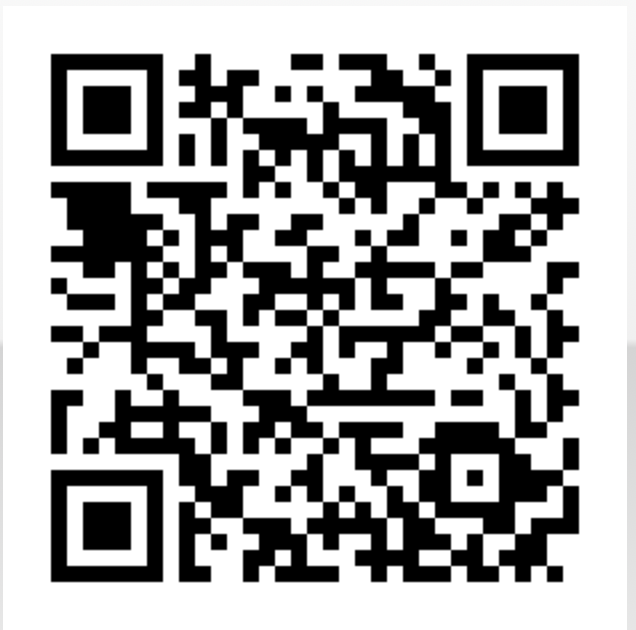
\includegraphics[height=15mm, width=15mm]{genetopo.png}
\end{wrapfigure}


演習の問題は授業ページ(\url{https://masataka123.github.io/2022_winter_generaltopology/})にもあります. 
右下のQRコードからを読み込んでも構いません.

\begin{comment}
\item コンパクト集合$A,B$とする
\begin{enumerate}
\item $A \cap B$はコンパクト集合か?
\item $B$が閉集合ならば$A \cap  B$はコンパクトである
\item $X$がハウスドルフならば$A \cap B$はコンパクトになることをしめせ. 
\end{enumerate}

\item $X$を集合とし, $\mathscr{O}_1, \mathscr{O}_2$を $\mathscr{O}_1 \subset \mathscr{O}_2$となる開集合系とする. 次の問いに答えよ.\footnote{開集合が多ければハウスドルフになりやすく, 開集合が少なければコンパクトになりやすいということである.}
\begin{enumerate}
\item 位相空間$(X, \mathscr{O}_1)$がハウスドルフならば, 位相空間$(X, \mathscr{O}_2)$もハウスドルフである.
\item 位相空間$(X, \mathscr{O}_2)$がコンパクトならば, 位相空間$(X, \mathscr{O}_1)$もコンパクトである.
\end{enumerate}
\end{comment}



 \end{document}
